\documentclass[xcolor=dvipsnames,aspectratio=169,13pt]{beamer} %Other possible values are: 1610, 149, 54, 43 and 32.
\usepackage{siunitx} %% Sistema Internacional de Unidades
\usepackage{multicol}
\usepackage{graphicx}
\usepackage{subfigmat}
\usepackage{changepage}
\usepackage{hyperref}
\usepackage{amsfonts}
\usepackage{ragged2e}



\usepackage[utf8]{inputenc} % codificacao de caracteres
\usepackage[T1]{fontenc}    % codificacao de fontes
%\usepackage[brazil]{babel}   % Habilita a língua portuguesa

%\usepackage{refcheck}
\usepackage{biblatex}

\usepackage{pgf,tikz,pgfplots,pgfkeys}
\pgfplotsset{compat=1.15}
\usetikzlibrary{arrows, calc, automata}

\DeclareMathOperator{\tr}{tr}

\usepackage{booktabs}
\usepackage[scale=2]{ccicons}

\mode<presentation>
\usetheme{metropolis}
\setbeamercovered{transparent}

\usepackage{xspace}
\newcommand{\themename}{\textbf{\textsc{metropolis}}\xspace}
\usepackage{booktabs}
\usepackage[scale=2]{ccicons}
\newcommand{\myscaleF}{0.38}
\newcommand{\myscale}{0.29}

\usefonttheme[onlymath]{serif}
\usefonttheme{structurebold} % fonte modo matematico


%  Define as cores a serem usadas
\definecolor{UFGblue}{rgb}{0.0039, 0.3529, 0.6431} 
\definecolor{UFGred}{HTML}{990000}
\definecolor{UFGorange}{rgb}{0.9216, 0.4863, 0.0784}
\definecolor{UFGgreen}{rgb}{0.0509, 0.4509, 0.1568}
\definecolor{UFGgrey}{rgb}{0.3686, 0.5255, 0.6235} % UBC Grey (secondary)
\definecolor{ultramarine}{rgb}{0, 0.125, 0.376} 
\definecolor{UFGorange}{rgb}{0.9216, 0.4863, 0.0784}%{HTML}{EB811B}
\definecolor{UFGgreen}{rgb}{0.0509, 0.4509, 0.1568}
\definecolor{UFGred}{HTML}{990000}

\definecolor{mLightBrown}{HTML}{990000} % alert block
\definecolor{mLightGreen}{HTML}{EB811B} % example text


%Colocando um marca dagua
\setbeamertemplate{background}{\tikz[overlay,remember picture]
  \node[opacity=.04]at (current page.center){
    
\includegraphics[width=7cm]{ufglogo.png}};}


% - Define a cor da página
\setbeamercolor{background canvas}{bg=UFGblue!5}

% Define a cor da letra
\setbeamercolor{normal text}{fg=black}
%\setbeamercolor{example text}{fg=UFGgreen}
%\setbeamercolor{alerted text}{fg=UFGorange}



% Definindo as cores do palette
\setbeamercolor{palette primary}{bg= UFGblue!30 ,fg=UFGblue!90!black}
%\setbeamercolor{palette secondary}{bg=UFGblue,fg=white}
%\setbeamercolor{palette tertiary}{bg=UFGlue,fg=white}
%\setbeamercolor{palette quaternary}{bg=UFGblue,fg=white}l%


% tirando a cor dos cabeçalhos dos blocks
 \setbeamercolor{block title}{bg= }
 \setbeamercolor{block title example}{bg=}
 \setbeamercolor{block title alerted}{bg=}




% \setbeamercolor{structure}{fg=UFGblue} % itemize, enumerate, etc
% \setbeamercolor{section in toc}{fg=UFGblue} % TOC sections
% \setbeamercolor{title}{bg=UFGgrey}
% \setbeamercolor{item}{fg=green}

% \setbeamercolor{block body alerted}{bg=alerted text.fg!10}
% \setbeamercolor{block body}{bg=UFGblue!20}
% \setbeamercolor{block body example}{bg=UFGgreen!20}
 %\setbeamercolor{block body alerted}{bg=UFGblue!10}
% \setbeamercolor{block title alerted}{bg=UFGred, fg=white}


% Transparencia dos blocks
%\addtobeamertemplate{block begin}{\pgfsetfillopacity{1}}{\pgfsetfillopacity{1}}
%\addtobeamertemplate{block alerted begin}{\pgfsetfillopacity{1}}{\pgfsetfillopacity{1}}
%\addtobeamertemplate{block example begin}{\pgfsetfillopacity{1}}{\pgfsetfillopacity{1}}


% % Override palette coloring with secondary
% \setbeamercolor{subsection in head/foot}{bg=UFGblue,fg=white}
% \setbeamercolor{section in head/foot}{bg=UFGgreen,fg=white}
% \setbeamertemplate{enumerate items}[default]
% \setbeamercolor{enumerate item}{fg=UFGblue}


% Definicao de novos comandos
\providecommand{\sin}{} \renewcommand{\sin}{\hspace{2pt}\textrm{sen \!}}
\providecommand{\sinh}{} \renewcommand{\sinh}{\hspace{2pt}\textrm{senh \!}}
%\providecommand{\tan}{} \renewcommand{\tan}{\hspace{2pt}\textrm{tan}}
\newcommand{\R}{\mathbb{R}}

\newtheorem{proposition}[theorem]{Proposition}



% Desativando o cabeçalho
%\setbeamertemplate{headline}{}

% Colocando numero de paginas no slide
\setbeamertemplate{footline}{}

% Tela cheia
%\hypersetup{pdfpagemode=FullScreen}

% justificando o texto nos blocks
\addtobeamertemplate{block begin}{}{\justifying}  %new code
\addtobeamertemplate{block example begin}{}{\justifying}  %new code
\addtobeamertemplate{block alerted begin}{}{\justifying}  %new code

% justificando o texto fora dos blocks
\apptocmd{\frame}{}{\justifying}{}

\setbeamertemplate{itemize body end}{\vspace{2em}}


%-----------------------------------------------------------------------

\title
  {
    On the inexact scaled gradient projection method
  }

\author[M. ~Lemes] % (optional, use only with lots of authors)
  {
   \textbf{Max ~Lemes}\\
   Universidade Federal de Goiás, Brazil
  }

 \institute[Federal University of Goiás] % (optional, but mostly needed)
  {
   %Based on the joint work with: {\bf}, 
   Joint work with: \textbf{Orizon P. ~Ferreira (IME/UFG)}, 
                    \textbf{Leandro F. Prudente (IME/UFG)}.
  }

\date[Goiânia  June 10,    2021]
  % (optional, should be abbreviation of conference name)
  {
    \textcolor{UFGorange}{\textbf{Seminário de Otimização do IME/UFG}}\\
    Goiânia - Brazil, June 10, 2021
  }

\subject
  {
    Continuous Optimization of IME/UFG
  }

%-----------------------------------------------------------------------
\addbibresource{Seminario.bib}
\begin{document}

\maketitle

\begin{frame}
  \frametitle{Outline}
  \tableofcontents
  % You might wish to add the option [pausesections]
\end{frame}


\section{The problem,  definitions and preliminaries results}


\begin{frame}
  \frametitle{The main problem}

  We want to present an inexact version of the scaled gradient projection method  for  \textcolor{UFGred}{constrained convex optimization problem} as follows

  \bigskip

  \begin{equation} \label{eq:OptP}
    \min \{ f(x) :~   x\in C\},
  \end{equation}

  \bigskip

  where $C$ is a closed and convex subset of $\mathbb{R}^n$ and $f:\mathbb{R}^n \to \mathbb{R}$ is a continuously differentiable function.


\end{frame}


\begin{frame}
  \frametitle{Scaled Gradient Projection Method\footfullcite{Bonettini2009}}

  \begin{enumerate}
    \item[Step 0.] Choose  $\sigma, \tau \in (0, 1)$, $0 < \alpha_{\min} \leq \alpha_{\max}$. Let $x^0\in C$ and set $k=0$;

    \item[Step 1.] Choose $\alpha_k\in [\alpha_{\min}, \alpha_{\max}]$ and a positive definite matrix $D_k$ and take  $w^{k}\in C$  as
      \begin{equation*}
        w^k := {\cal P}_{C}^{D_k} (x^{k}-\alpha_k D_k^{-1}\nabla f(x^{k}))
      \end{equation*}

      If $w^k= x^k$, then {\bf stop}; otherwise,
    \item [Step 2.] Choose $\tau_k$ and define the next iterate $x^{k+1}$ as
          \begin{equation} \label{eq:IterArm}
            x^{k+1} = x^{k} + \tau_k (w^k - x^{k}).
          \end{equation}
          and go back to the Step 1.
  \end{enumerate}
\end{frame}


\begin{frame}
  \frametitle{Scaled Gradient Projection Method}
  Let  $D$ be a $n\times n$ positive definite matrix and $\| \cdot \|_{D} : \mathbb{R}^{n}\rightarrow \mathbb{R}$ be  the norm  defined by
  \begin{equation*} 
    \|d\|_{D}:=\sqrt{\left\langle D d,d\right\rangle},\quad \forall d\in \mathbb{R}^{n}.
  \end{equation*}
  For a fixed  constant $\mu \geq 1$,  {\it denote by  ${\cal D}_{\mu}$  the set of symmetric positive definite matrices $n\times n$ with all eigenvalues contained in the interval $[\frac{1}{\mu}, \mu]$}.
  \begin{itemize}
    \item ${\cal D}_{\mu}$   is compact;
    \item If $D\in {\cal D}_{\mu}$, it follows that $D^{-1}$ also belongs to $ {\cal D}_{\mu}$;
    \item $\forall D\in {\cal D}_{\mu}$,  we obtain
          \begin{equation*} 
            \frac{1}{\mu}\|d\|^2\leq \|d\|^2_{D}\leq \mu \|d\|^2, \qquad \forall d\in \mathbb{R}^n.
          \end{equation*}
  \end{itemize}
\end{frame}


% \begin{frame}
%   \frametitle{Preliminaries}

%   \begin{definition}
%     Let $(y^k)_{k\in\mathbb{N}}$ be a sequence in $\mathbb{R}^n$ and   $(D_k)_{k\in\mathbb{N}}$ be  a sequence in ${\cal D}_{\mu}$.  The sequence $(y^k)_{k\in\mathbb{N}}$ is said to be \textcolor{UFGred}{quasi-Fej\'er convergent} to a set $W\subset \mathbb{R}^n$ with respect to  $(D_k)_{k\in\mathbb{N}}$ if, for  all $w\in W$, there exists a sequence $(\epsilon_k)_{k\in\mathbb{N}}\subset\mathbb{R}$ such that $\epsilon_k\geq 0$, $\displaystyle\sum_{k\in \mathbb{N}}\epsilon_k<\infty$, and
%     \[
%       \|y^{k+1}-w\|_{D_{k+1}}^2\leq \|y^k-w\|_{D_k}^2+\epsilon_k,
%     \]
%     for all $k\in \mathbb{N}$.
%   \end{definition}
% \end{frame}


% \begin{frame}
%   \frametitle{Preliminaries}

%   \begin{theorem}
%     Let $(y^k)_{k\in\mathbb{N}}$ be a sequence in $\mathbb{R}^n$ and   $(D_k)_{k\in\mathbb{N}}$ be  a sequence in ${\cal D}_{\mu}$.   If $(y^k)_{k\in\mathbb{N}}$ is quasi-Fej\'er convergent to a nomempty set $W\subset  \mathbb{R}^n$ with respect to $(D_k)_{k\in\mathbb{N}}$, then $(y^k)_{k\in\mathbb{N}}$ is \textcolor{UFGred}{bounded}. Furthermore, if a \textcolor{UFGred}{cluster point ${\bar y}$} of $(y^k)_{k\in\mathbb{N}}$ belongs to $W$, then $\displaystyle\lim_{k\rightarrow\infty}y^k={\bar y}$.
%   \end{theorem}
% \end{frame}

\begin{frame}
  \frametitle{Exact Projection}

  \begin{definition}
    The \textcolor{UFGred}{exact  projection} of the point $v\in \mathbb{R}^{n}$ onto $C$ with respect to the norm $\| \cdot \| _{D}$, denoted by  ${\cal P}_{C}^{D}(v)$, is  defined~by
    \begin{equation*}
      {\cal P}_{C}^{D}(v):=\arg \min _{z\in C}\|z-v\|^2_{D}.
    \end{equation*}
  \end{definition}

  \begin{lemma}
    Let $v, w \in {\mathbb R}^n$.  Then,  $w={\cal P}_{C}^{D}(v)$ if and only if  $w\in C$ and
    \[
      \left\langle D(v-w), y-w\right\rangle \leq  0,
    \]
    for all $y \in C.$
  \end{lemma}

\end{frame}


\begin{frame}
  \frametitle{Inexact Projections\footfullcite{BirginMartinezRaydan2003}}

  \begin{definition}
    The \textcolor{UFGred}{feasible inexact projection mapping}, with respect to the norm $\| \cdot \|_{D}$,   onto $C$  relative to a point  $u \in C$ and forcing parameter $\zeta\in (0, 1]$, denoted by ${\cal P}_{C,\zeta}^{D}(u,  \cdot): {\mathbb R}^n \rightrightarrows C$,  is the set-valued mapping defined as follows
    \begin{equation*}
      {\cal P}_{C,\zeta}^{D}(u, v) := \left\{w\in C:~ \|w-v\|_{D}^2\leq \zeta \| {\cal P}_{C}^{D}(v)-v\|_{D}^2+(1-\zeta)\|u-v\|_{D}^2 \right\}.
    \end{equation*}
    Each point $w\in {\cal P}_{C,\zeta}^{D}(u, v) $ is called a  \textcolor{UFGred}{feasible inexact projection},  with respect to the norm $\| \cdot \|_{D}$,  of $v$ onto $C$ relative to $u$ and forcing parameter $\zeta\in (0, 1]$.
  \end{definition}
\end{frame}




\begin{frame}[t]\frametitle{Inexact Projections\footfullcite{OrizonFabianaGilson2018}}
  \begin{definition}
    The \textcolor{UFGred}{feasible inexact projection mapping}, with respect to the norm $\| \cdot \|_{D}$,  onto $C$ relative to $u \in C$ and forcing parameter $\gamma\geq 0$, denoted by ${\cal R}_{C,\gamma}^{D}(u, \cdot): {\mathbb R}^n \rightrightarrows C$,  is the set-valued mapping defined as follows
    \begin{equation*} 
      {\cal R}_{C,\gamma}^{D}(u, v):= \left\{w\in C:~\left\langle D(v-w), y-w \right\rangle \leq \gamma \|w-u\|_{D}^2, \quad \forall~ y \in C \right\}.
    \end{equation*}
    Each point $w\in {\cal R}_{C,\gamma}^{D}(u, v)$ is called a feasible inexact projection,  with respect to the norm $\| \cdot \|_{D}$,  of $v$ onto $C$ relative to $u$ and forcing parameter $\gamma\geq 0$.
  \end{definition}
\end{frame}





\begin{frame}[t]\frametitle{Inexact Projections}
  \begin{lemma}
    Let $v \in {\mathbb R}^n$, $u \in C$, $\gamma \geq 0$  and $\zeta\in (0, 1]$.  If  $0 \leq \gamma <1/2$ and $\zeta=1-2\gamma$, then
    \[
      {\cal R}_{C,\gamma}^{D}(u, v) \subset {\cal P}_{C,\zeta}^{D}(u, v).
    \]
  \end{lemma}

  \begin{proposition}
    Let $v \in {\mathbb R}^n$, $u \in C$ and assume that $C$ is a bounded set. Then, for each $0<\gamma < 1/2$,     there exist $0 < \zeta  <1$ such that
    \[
      {\cal P}_{C,\zeta}^{D}(u, v)  \subseteq    {\cal R}_{C,\gamma}^{D}(u, v)
    \]
  \end{proposition}
\end{frame}


\begin{frame}[t]\frametitle{Inexact Projections}
  \begin{lemma}
    Let $x \in C$, $\alpha > 0$ and  $z(\alpha) = x-\alpha D^{-1} \nabla f(x)$. Take $w(\alpha) \in  {\cal P}_{C,\zeta}^{D}(x, z(\alpha))$ with $\zeta\in (0, 1]$. Then, there hold
    \begin{enumerate}[(i)]
      \item {\small $\displaystyle \langle \nabla f(x), w(\alpha) - x\rangle \leq -\frac{1}{2\alpha} \|w(\alpha) -x\|_{D}^2 +   \frac{\zeta}{2\alpha} \left[\| {\cal P}_{C}^{D}(z(\alpha))-z(\alpha)\|_{D}^2 - \|x-z(\alpha)\|_{D}^2\right]$;}

      \item the point $x$ is stationary for problem \eqref{eq:OptP} if, and only if, $x \in {\cal P}_{C,\zeta}^{D}(x, z(\alpha))$;

      \item if  $x \in C$ is a nonstationary point for problem \eqref{eq:OptP}, then $\Big\langle \nabla f(x), w(\alpha) - x \Big\rangle < 0$. Equivalently, if there exists ${\bar \alpha}>0$ such that $\Big\langle \nabla f(x), w({\bar \alpha}) - x \Big\rangle \geq 0$, then $x$ is stationary for problem \eqref{eq:OptP}.
    \end{enumerate}
  \end{lemma}
\end{frame}


\section{Inexact scaled gradient method}

\begingroup
\small
\begin{frame}[t]
  \frametitle{InexProj-SGM employing nonmonotone line search}

  \begin{enumerate}
    \item[Step 0.] Choose  $\sigma,{\zeta_{\min}}  \in (0, 1)$, $0 < \alpha_{\min} \leq \alpha_{\max}$ and $\mu \geq1$. Let $x^0\in C$, $\nu_0\geq 0$ and set $k\gets0$.

    \item[Step 1.] Choose positive real numbers $\alpha_k$ and $\zeta_k$ and a positive definite matrix $D_k$ such that
      \begin{equation*} 
        \alpha_{\min}\leq \alpha_k \leq \alpha_{\max}, \qquad \qquad 0 <{\zeta_{\min}}<\zeta_k \leq 1, \qquad \qquad D_k\in {\cal D}_{\mu}.
      \end{equation*}
      Compute  $w^{k}\in C$  as any feasible inexact projection  with respect to the norm $\| \cdot \| _{D_k}$ of 
      \[
        z^k := x^{k}-\alpha_k D_k^{-1}\nabla f(x^{k})
      \]
      onto $C$ relative to $x^{k}$  with forcing parameter $\zeta_k$, i.e.,
      \begin{equation*} 
        w^k \in   {\cal P}_{C, \zeta_k}^{D_k}(x^{k}, z^k).
      \end{equation*}
      If $w^k= x^k$, then {\bf stop} declaring convergence.
  \end{enumerate}
\end{frame}
\endgroup


\begingroup
\small
\begin{frame}[t]
  \frametitle{InexProj-SGM employing nonmonotone line search}

  \begin{enumerate}
    \item[Step 2.] Set $\tau_{\textrm{trial}} \gets 1$. If
    \begin{equation}\label{eq:TkArm}
       f\Big(x^{k}+ \tau_{\textrm{trial}}(w^k - x^{k})\Big) \leq f(x^{k}) + \sigma \tau_{\textrm{trial}}\Big\langle \nabla f(x^{k}), w^k - x^{k} \Big\rangle + \nu_k,
    \end{equation}
    then  $\tau_k\gets \tau_{\textrm{trial}}$, define the next iterate $x^{k+1}$ as
    \begin{equation} \label{eq:IterArm}
      x^{k+1} = x^{k} + \tau_k (w^k - x^{k}),
    \end{equation}
    and go to {\bf Step 3}. Otherwise, choose $\tau_{\textrm{new}} \in [\underline\omega \tau_{\textrm{trial}}, \bar\omega \tau_{\textrm{trial}} ]$, set $\tau_{\textrm{trial}} \gets \tau_{\textrm{new}}$, and repeat test \eqref{eq:TkArm}.
    
    \item [Step 3.] Take  $\delta_{k+1}\in [\delta_{\min}, 1]$ and choose    $\nu_{k+1}\in {\mathbb R}$ satisfying
    \begin{equation*} 
      0\leq \nu_{k+1}\leq (1-\delta_{k+1})\Big[f(x^{k})+\nu_{k}-f(x^{k+1})\Big].
    \end{equation*}
    Set $k\gets k+1$ and go to \textbf{Step~1}.
  \end{enumerate}
\end{frame}
\endgroup

\begin{frame}[t]\frametitle{Nonmonotone line search}
  \begin{block}{Remarks}
  There are several ways of choosing $\nu_k$
    \begin{enumerate}[(i)]
      \item If $\nu_k = 0$, the line search (\ref{eq:IterArm}) is the well-known Armijo line search.
      \item If $f_{\max} = \max\{f(x^{k-j})\, | \, 0\leq j\leq \min\{k,M\}\}$ and
            \begin{equation}\label{eq:nuGLL}
              \nu_k = f_{\max} - f(x^k)
            \end{equation}
            the line search (\ref{eq:IterArm}) is the same defined by Grippo, Lampariello and Lucidi\footfullcite{Grippo1986}.
    \end{enumerate}
  \end{block}
\end{frame}

\begin{frame}[t]\frametitle{Nonmonotone line search}
  \begin{block}{}
    \begin{enumerate}[(iii)]
      \item Let   $0\leq \eta_{min}\leq \eta_{max}<1$,   $c_0 = f(x_0)$ and  $q_0 = 1$. Choose $\eta_k\in [\eta_{min},  \eta_{max}]$ and set
            \begin{equation*}
              q_{k+1}=\eta_kq_{k}+1, \qquad c_{k+1} = (\eta_k q_k c_k + f(x^{k+1}))/q_{k+1}, \qquad \forall k \in \mathbb{N}.
            \end{equation*}
            If $\delta_{k+1}=1/q_{k+1}$ and
            \begin{equation}\label{eq:nuZH}
              \nu_{k}=c_k-f(x^k)
            \end{equation}
            the line search \eqref{eq:IterArm} is the same defined by Zhang and Hager\footfullcite{ZhangHager2004}.
    \end{enumerate}
  \end{block}
\end{frame}



\section{Partial asymptotic convergence}


\begin{frame}[t]\frametitle{Partial asymptotic convergence analysis}
  \begin{lemma}
    There holds  $0\leq \delta_{k+1}\Big[ f(x^{k})+\nu_{k}-  f(x^{k+1})\Big] \leq \Big( f(x^{k})+\nu_{k}\Big) - \Big( f(x^{k+1})+\nu_{k+1}\Big)$, for all $k \in \mathbb{N}$. As consequence the sequence   $\left(f(x^k)+\nu_k\right)_{k\in\mathbb{N}}$ is    non-increasing.
  \end{lemma}

  \bigskip
  \bigskip



  \begin{theorem} 
    Assume that $\displaystyle\lim_{k\to +\infty} \nu_{k} = 0$.   Then, Algorithm InexProj-SGM stops in a finite number of iterations at a stationary point of problem~\eqref{eq:OptP}, or generates an infinite sequence $(x^k)_{k\in\mathbb{N}}$ for which every cluster point is stationary for problem~\eqref{eq:OptP}.
  \end{theorem}
\end{frame}


\begin{frame}[t]\frametitle{Partial asymptotic convergence analysis}
  \begin{proposition}
    If $\delta_{min}>0$,  then  $\displaystyle\sum_{k=0}^{+\infty} \nu_k<+\infty$. Consequently, $\displaystyle\lim_{k\to +\infty} \nu_{k} = 0$.\footfullcite{GrapigliaSachs2017}
  \end{proposition}

  \begin{block}{Remark}
    Armijo line search and nonmonotone line search strategy defined by \eqref{eq:nuZH} satisfies  a condition $\delta_{min}>0$.  However,    for  the  nonmonotone line search strategy proposed by \eqref{eq:nuGLL},  we   can only guarantee that $\delta_{min}\geq 0$. Hence,  we need deal with this case separately.
  \end{block}
\end{frame}



\begin{frame}\frametitle{Partial asymptotic convergence analysis}
  \begin{proposition}
    Assume that the sequence  $(x^k)_{k\in\mathbb{N}}$ is generated by Algorithm~InexProj-SGM with the  nonmonotone line  search \eqref{eq:nuGLL}, i.e.,  $\nu_{k}= f_{\max}-f(x^k)$ for all  $k \in \mathbb{N}$. In addition,  assume that the level set $C_{0}:=\{ x\in C: ~ f(x)\leq f(x^0) \}$ is bounded and $\nu_0= 0$.  Then, $\displaystyle\lim_{k\to +\infty} \nu_{k} = 0$.
  \end{proposition}
\end{frame}


\section{Full asymptotic convergence}


\begin{frame}[t]\frametitle{Full asymptotic convergence analysis}
  We will prove, under suitable assumptions, the full convergence of the  sequence $(x^k)_{k\in\mathbb{N}}$.  For this end,  we   assume  that in ${\bf Step\,1}$  of  Algorithm~InexProj-SGM:
  \begin{itemize}
    \item[{\bf A1.}] For all $k \in \mathbb{N}$, we take   $w^k \in   {\cal R}_{C,\gamma_k}^{D_k}(x^{k}, z^k)$   with $\gamma_k=(1-\zeta_k)/2$.
      \item[{\bf A2.}]For all $k \in \mathbb{N}$,  we take  $0\leq \nu_{k}$ such that  $\sum_{k=0}^{+\infty} \nu_k<+\infty$.
  \end{itemize}
  Armijo line search and nonmonotone line search strategies defined by \eqref{eq:nuZH} satisfies  the assumption {\bf A2}. 

\end{frame}


\begin{frame}[c]\frametitle{Full asymptotic convergence analysis}
 \begin{lemma}
  For each  $x\in C$, there holds
  \begin{equation*}
    \|x^{k+1}-x\|_{D_k}^2 \leq \|x^k-x\|_{D_k}^2 + 2\alpha_k\tau_k \Big\langle \nabla f(x^k), x-x^k\Big\rangle + \xi \Big[f(x^k) - f(x^{k+1})+ \nu_k \Big], \quad \forall ~k \in \mathbb{N}.
  \end{equation*}
  where $\xi := \dfrac{2 \alpha_{\max}}{\sigma} > 0.$
\end{lemma}
\begin{corollary}
  Assume that $f$ is a convex function. If $U := \left\{x \in C: f(x) \leq \inf_{k\in {\mathbb N}}\left(f(x^{k})+\nu_k\right) \right\}$ is not empty, then $(x^k)_{k\in\mathbb{N}}$ converges to a stationary point of problem~\eqref{eq:OptP}.
\end{corollary}
\end{frame}


\begin{frame}[t]\frametitle{Full asymptotic convergence analysis}


\begin{theorem}
  If $f$ is a convex function and $(x^k)_{k\in\mathbb{N}}$ has no cluster points,  then $\Omega^* = \varnothing$, $\lim_{k \to \infty} \|x^k\|=~+\infty$, and $\inf_{k\in {\mathbb N}} f(x^k) = \inf \{f(x) : x \in C\}$.
\end{theorem}
\end{frame}


\begin{frame}[t]\frametitle{Full asymptotic convergence analysis}
\begin{corollary}
  If $f$ is a convex function and $(x^k)_{k\in\mathbb{N}}$ has at least one cluster point, then    $(x^k)_{k\in\mathbb{N}}$ converges to a stationary point of problem~\eqref{eq:OptP}.
\end{corollary}

\end{frame}


\begin{frame}[t]\frametitle{Full asymptotic convergence analysis}
\begin{theorem}
  Assume that $f$ is a convex function and  $\Omega^* \neq \varnothing$. Then,   $(x^k)_{k\in\mathbb{N}}$ converge to an optimal solution of problem~\eqref{eq:OptP}.
\end{theorem}
\end{frame}


\section{Iteration-complexity bound}


\begin{frame}[t]\frametitle{Interation-complexity bound}
    Besides  assuming   that  in ${\bf Step\,1}$ of  Algorithm~InexProj-SGM we take   $(x^k)_{k\in\mathbb{N}}$ satisfying {\bf A1} and {\bf A2},  we also need the following assumption.
\begin{itemize}
  \item[{\bf A3.}] The  gradient $\nabla f$ of $f$ is  Lipschitz continuous with constant $L>0$.
\end{itemize}


\begin{lemma}
  The steepsize $\tau_k$ in Algorithm~InexProj-SGM satisfies $\tau_k \geq \tau_{\min}$,
\end{lemma}
where 
\begin{equation*}
  \tau_{\min} := \min \left\{1, \frac{\tau(1-\sigma)}{{\alpha_{\max}}\mu L}\right\}.
\end{equation*}
\end{frame}


\begin{frame}[t]\frametitle{Interation-complexity bound}
\begin{theorem} 
  For every $N \in \mathbb{N}$, the following inequality holds
  $$
    \min\left\{\|w^k-x^k\| :~ k= 0, 1 \ldots, N-1\right\} \leq \sqrt{\frac{2{\alpha_{\max}}\mu\left(f(x^0)-f^* +\sum_{k= 0}^{\infty}\nu_k\right) }{\sigma \tau_{\min}}} \frac{1}{\sqrt{N}}.
  $$
\end{theorem}

\begin{theorem} 
  Let $f$ be a convex function on $C$. Then, for every $N \in \mathbb{N}$, there holds
  $$
    \min \left\{f(x^k) - f^* :~k = 0, 1 \ldots, N-1\right\} \leq \frac{\|x^0 - x^*\|^2_{D_0} + \xi\left[f(x^0)-f^*+ \sum_{k=0}^{\infty} \nu_k\right]}{2 \alpha_{\min} \tau_{\min}}\frac{1}{N}.
  $$
\end{theorem}
\end{frame}

\begin{frame}[c]\frametitle{Interation-complexity bound}
  \begin{lemma} 
  Let $N_{k}$ be  the number of function evaluations after $k\geq 1$ iterations of Algorithm~InexProj-SGM. Then,  
  \[N_{k}\leq 1+ (k+1)\left[\frac{\log (\tau_{\min})}{\log(\tau)}+1 \right].\]
\end{lemma}
\end{frame}


\begin{frame}[c]\frametitle{Interation-complexity bound}
\begin{theorem}
  For a given $\epsilon>0$, the number  of  function evaluations in  Algorithm~InexProj-SGM are  at most
    $$
      1+\left({\frac{2{\alpha_{\max}}\mu\left(f(x^0)-f^* +\sum_{k= 0}^{\infty}\nu_k\right) }{\sigma \tau_{\min}}} \frac{1}{\epsilon^2}+1\right) \left(\frac{\log (\tau_{\min})}{\log (\tau)}+1\right),
    $$
  to compute $x^k$ and $w^k$ such that $\|  w^{k}-x^{k}\|\leq \epsilon$.
\end{theorem}
\end{frame}


\begin{frame}[c]\frametitle{Interation-complexity bound}
\begin{theorem}
  Let $f$ be a convex function on $C$. For a given $\epsilon>0$, the number  of  function evaluations in  Algorithm~InexProj-SGM are  at most

  $$
    1+\left(\frac{\|x^0 - x^*\|^2_{D_0} + \xi\left(f(x^0)-f^*+ \sum_{k=0}^{\infty} \nu_k\right)}{2 \alpha_{\min} \tau_{\min}}\frac{1}{\epsilon}+1\right) \left(\frac{\log (\tau_{\min})}{\log (\tau)}+1\right),
  $$
  to compute $x^k$ such that $f(x^k) - f^*\leq \epsilon$.
\end{theorem}
\end{frame}

\section{Numerical experiments}

\begin{frame}[t]\frametitle{Numerical experiments}
  Given $A$ and $B$ two $m\times n$ matrices, with $m\geq n$, and $c\in\mathbb{R}$, we consider the matrix function $f:\mathbb{R}^{n\times n}\to\mathbb{R}$ given by:
$$f(X):=\dfrac{1}{2}\|AX-B\|^2_F + \sum_{i=1}^{n-1} \left[ c \left( X_{i+1,i+1}-X_{i,i}^2 \right)^2 + (1-X_{i,i})^2   \right],$$
which combines a least squares term with a Rosenbrock-type function. $X_{i,j}$ stands for the $ij$-element of the matrix $X$ and $\|\cdot\|_F$ denotes the Frobenius matrix norm, i.e., $\|A\|_F:=\sqrt{\langle A,A \rangle}$ where the inner product is given by $\langle A,B \rangle = \tr(A^TB)$. 
\end{frame}


\begin{frame}[t]\frametitle{Numerical experiments}
  \begin{block}{Problem I\footfullcite{BirginMartinezRaydan2003}:}
    \begin{equation*} 
      \begin{array}{cl}
        \displaystyle\min     & f(X)           \\
        \mbox{s.t.} & X \in SDD^+,   \\
                    & L\leq X\leq U,
      \end{array}
    \end{equation*}
      where $SDD^+$ is the cone of symmetric and diagonally dominant real matrices with positive diagonal, i.e., 
      \[
        SDD^+ :=\{X\in\mathbb{R}^{n\times n}\mid X=X^T, \; X_{i,i}\geq \displaystyle\sum_{j\neq i}|X_{i,j}| \; \forall i\},
      \]
     $L$ and $U$ are given $n\times n$ matrices, and  $L\leq X\leq U$ means that $L_{i,j} \leq X_{i,j} \leq U_{i,j}$ for all $i,j$.
\end{block}

\end{frame}


\begin{frame}[t]\frametitle{Numerical experiments}
  \begin{block}{Problem II\footfullcite{allen2017linear}\footfullcite{douglasprojected}:}
    \begin{equation*}
      \begin{array}{cl}
        \displaystyle\min   & f(X)                  \\
        \mbox{s.t.}         & X \in \mathbb{S}^n_+, \\
                            & \tr(X)=1,
      \end{array}
    \end{equation*}
    where $\mathbb{S}^n_+$ is the cone of symmetric and positive semidefinite real matrices. The feasible set of Problem II was known as {\it spectrahedron} and appears in several interesting applications.
  \end{block}
\end{frame}


\begin{frame}[t]\frametitle{Numerical experiments}

We are interested in the \textcolor{UFGred}{spectral gradient version of the SPG method}, so we set $D_k:=I$ for all $k$, $\alpha_0 := \min(\alpha_{\max}, \max(\alpha_{\min}, 1/ \| \nabla f(x^0) \|))$ and, for $k>0$,

\begin{equation*}
\alpha_k:=\left\{
  \begin{array}{ll}
    \displaystyle\min (\alpha_{\max},\max (\alpha_{\min},\langle s^k,s^k\rangle/\langle s^k,y^k\rangle)), & \mbox{if} \; \langle s^k,y^k\rangle > 0\\
    \alpha_{\max}, & \mbox{otherwise},
  \end{array}\right.
\end{equation*}
where $s^k:=X^k - X^{k-1}$, $y^k:=\nabla f(X^k) - \nabla f(X^{k-1})$, $\alpha_{\min}=10^{-10}$, and $\alpha_{\max}=10^{10}$.


Concerning the stopping criterion, all runs were stopped at an iterate $X^k$ declaring convergence if
$$\displaystyle \max_{i,j} (|X^k_{i,j}-W^k_{i,j}| )\leq 10^{-6},$$ 
where $W^k \in {\cal P}_{C, \zeta_k}^{D_k}(x^{k}, z^k)$.
\end{frame}


\begin{frame}[t]\frametitle{Influence of the inexact projection}
 \begin{figure}[H]\centering
  \begin{tabular}{ccc}
    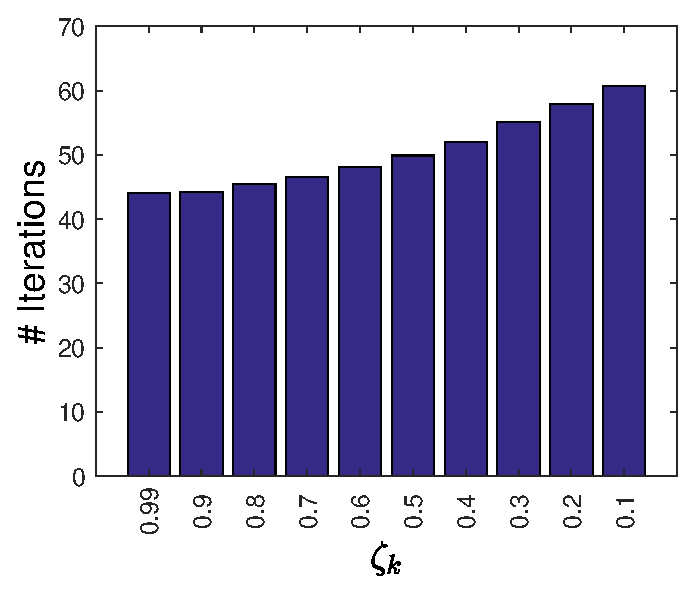
\includegraphics[scale=\myscaleF]{SDDit} & 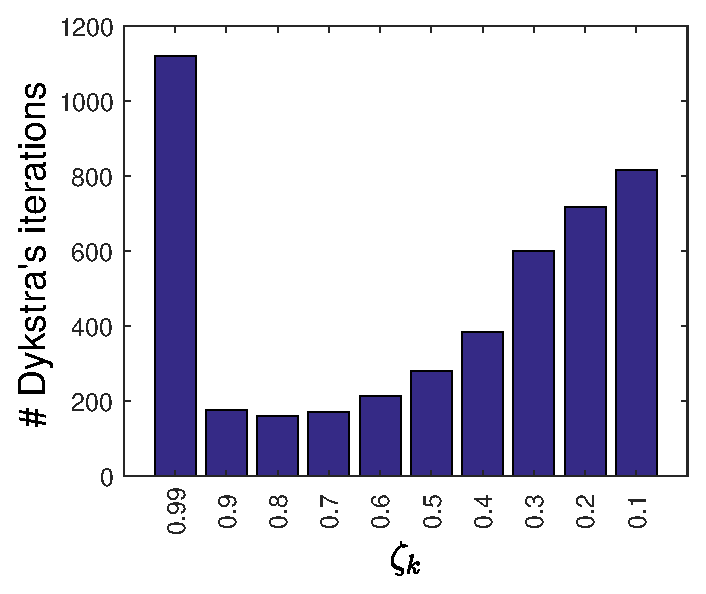
\includegraphics[scale=\myscaleF]{SDDDIT} & 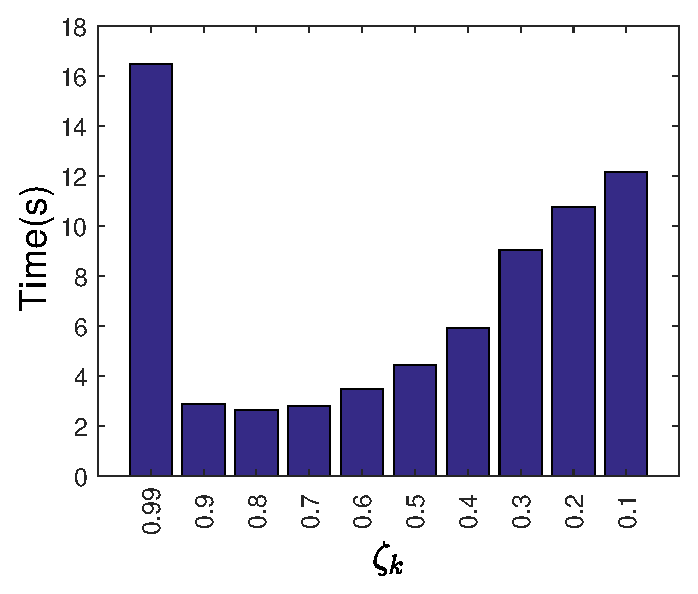
\includegraphics[scale=\myscaleF]{SDDtime}\\
    (a) & (b) & (c)\\
  \end{tabular}
  \caption{Results for 10 instances of Problem I using $n=100$, $m=200$, and $c=10$. Average number of: (a) iterations; (b) Dykstra’s iterations; (c)  CPU time in seconds needed to reach the solution for different choices of $\zeta_k$.}
\end{figure}   
\end{frame}

\begin{frame}[t]\frametitle{Influence of the inexact projection}    
\begin{figure}[H]\centering
  \begin{tabular}{ccc}
    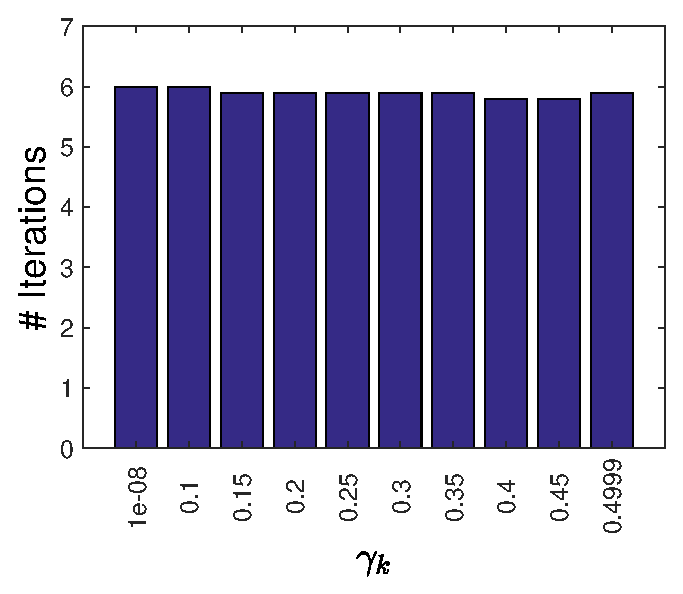
\includegraphics[scale=\myscaleF]{Specit} & 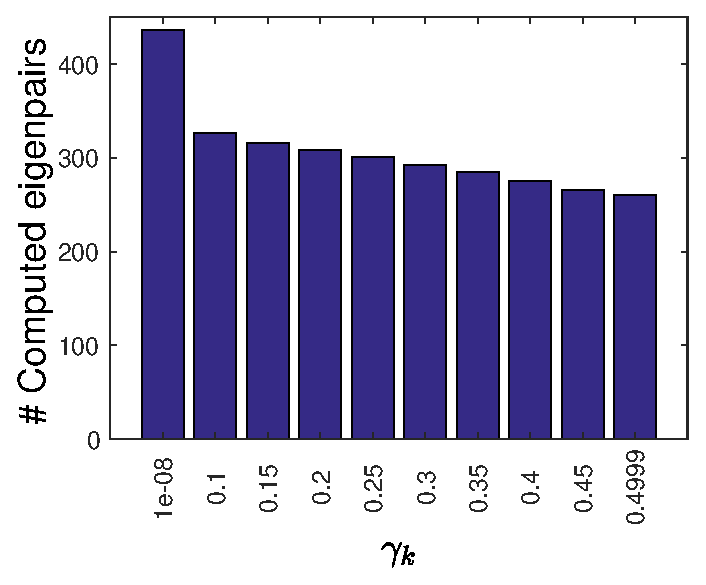
\includegraphics[scale=\myscaleF]{SpecFWIT} & 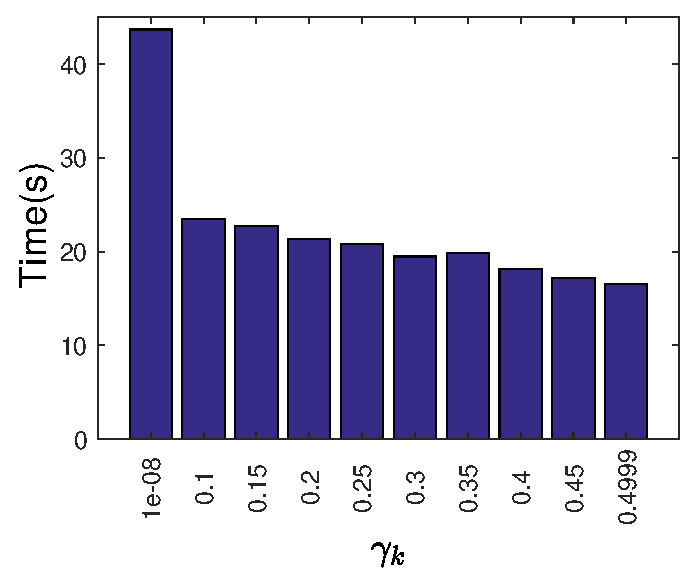
\includegraphics[scale=\myscaleF]{Spectime} \\
    (a) & (b) & (c)\\
  \end{tabular}
  \caption{Results for 10 instances of Problem II using $n=800$, $m=1000$, and $c=100$. Average number of: (a) iterations; (b) computed eigenpairs; (c)  CPU time in seconds needed to reach the solution for different choices of $\gamma_k$.}
\end{figure}
\end{frame}

\begin{frame}[t]\frametitle{Influence of the line search scheme}
    
\begin{figure}[H]\centering
  \begin{tabular}{cccc}
    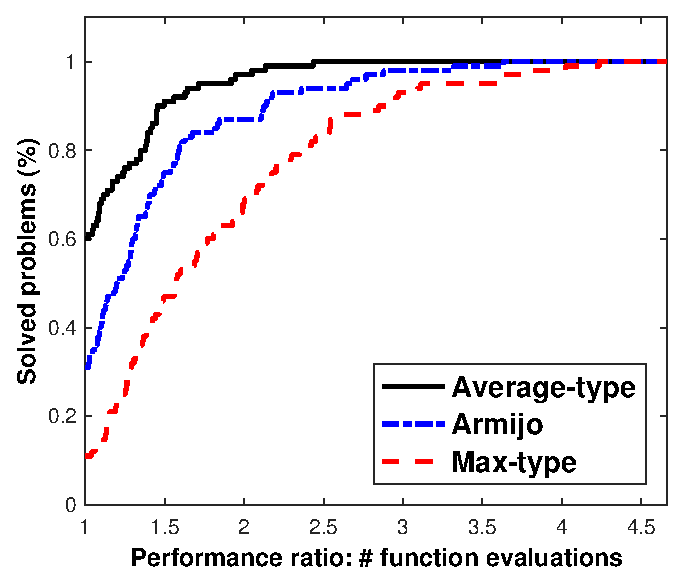
\includegraphics[scale=\myscale]{ppSDDnfev} &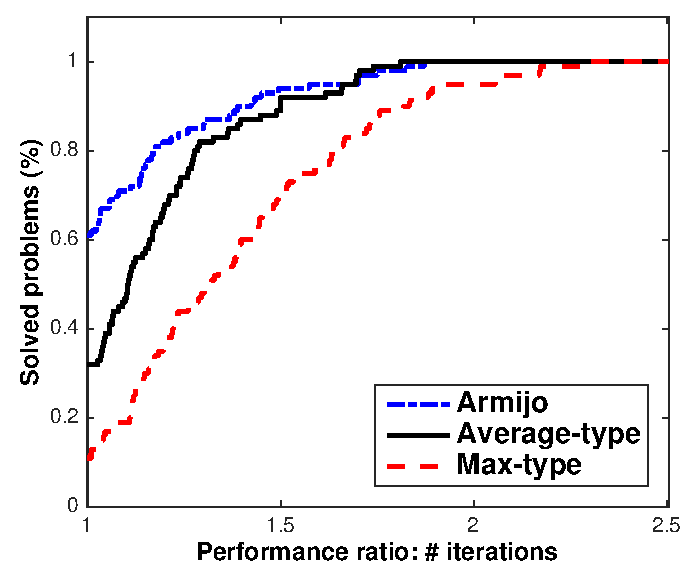
\includegraphics[scale=\myscale]{ppSDDit} & 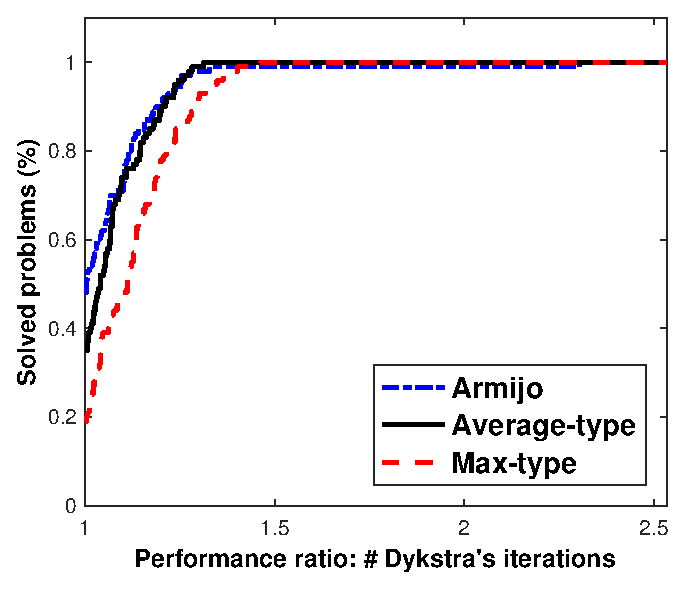
\includegraphics[scale=\myscale]{ppSDDnDIT} & 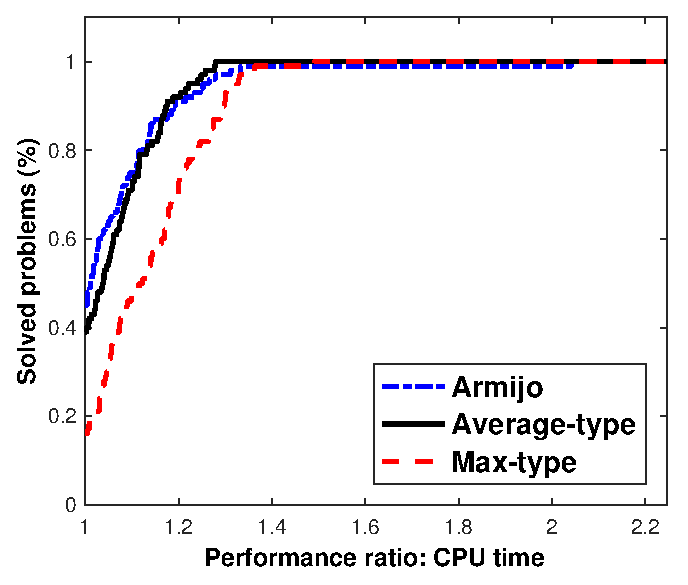
\includegraphics[scale=\myscale]{ppSDDtime} \\
    (a) & (b) & (c) & (d)\\
  \end{tabular}
  \caption{Performance profiles for Problem~I considering the SPG method with the Armijo, the Average-type, and the Max-type line searches strategies using as performance measurement: (a) number of function evaluations; (b) number of (outer) iterations; (c) number of Dykstra’s iterations; (d) CPU time.}
  
\end{figure}
\end{frame}

\begin{frame}[t]\frametitle{Influence of the line search scheme}
    \begin{figure}[H]\centering
  \begin{tabular}{cccc}
    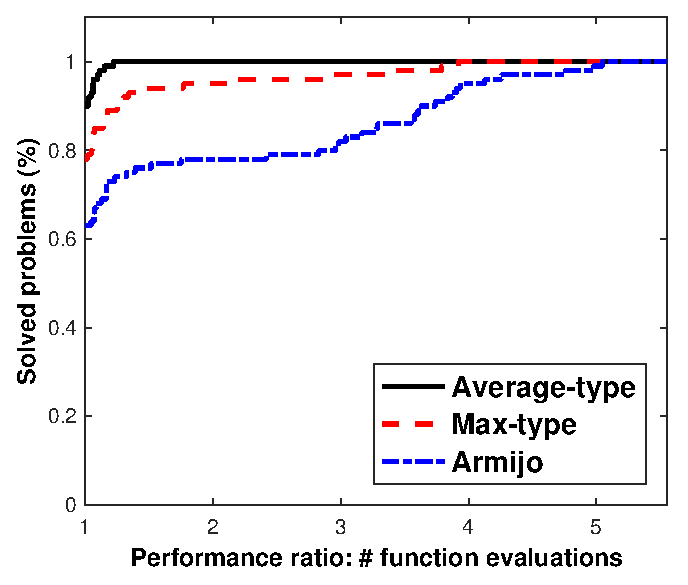
\includegraphics[scale=\myscale]{ppSpecnfev}&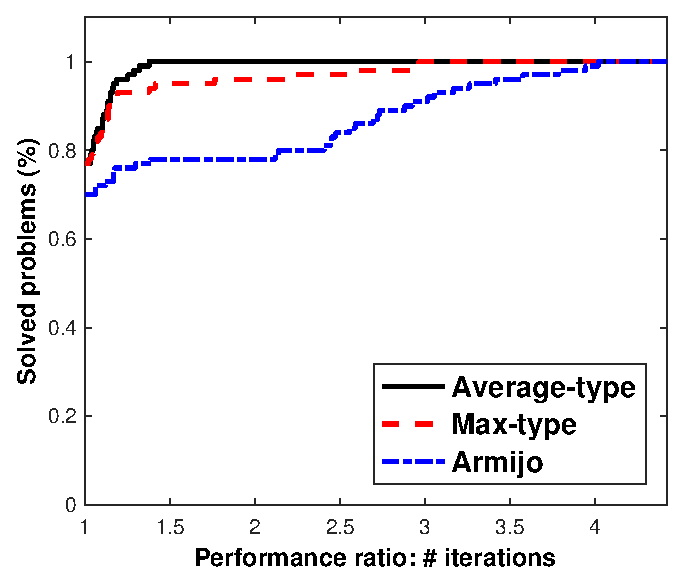
\includegraphics[scale=\myscale]{ppSpecit} & 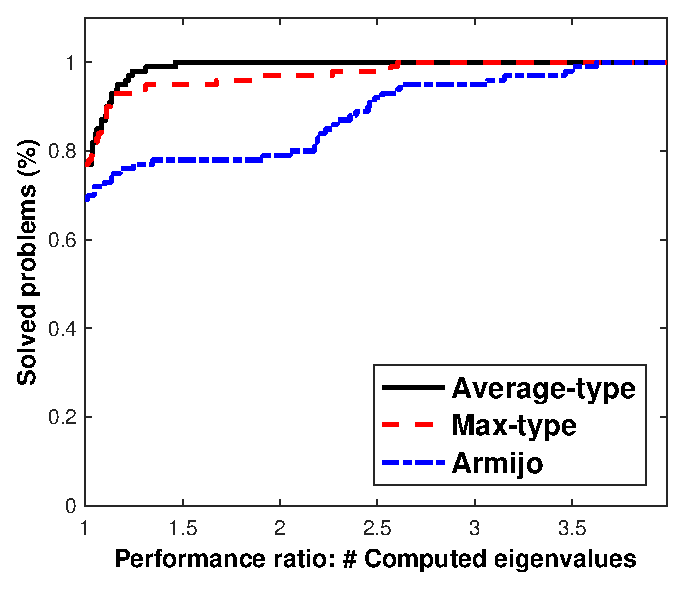
\includegraphics[scale=\myscale]{ppSpecnFW} & 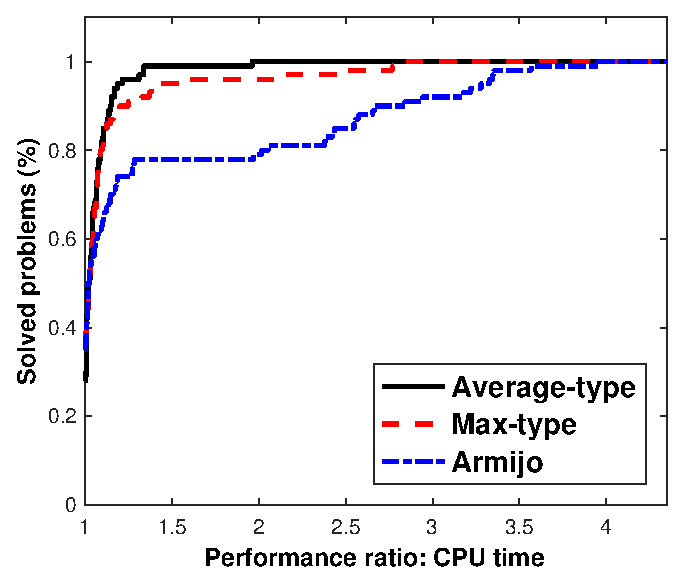
\includegraphics[scale=\myscale]{ppSpectime} \\
    (a) & (b) & (c) & (d)\\
  \end{tabular}
  \caption{Performance profiles for Problem~II considering the SPG method with the Armijo, the Average-type, and the Max-type line searches strategies using as performance measurement: (a) number of function evaluations; (b) number of (outer) iterations; (c) number of computed eigenpairs; (d) CPU time.}
\end{figure}
\end{frame}

\begin{frame}[c]\frametitle{}
 \begin{center}
  \Huge \textbf{Thank you!}
 \end{center}
\end{frame}

\end{document}